\PassOptionsToPackage{usenames,dvipsnames}{xcolor}
\documentclass[tikz,border=2]{standalone}
\usepackage{gillius2}
\renewcommand{\familydefault}{\sfdefault}
%% \usepackage{lmodern} % enhanced version of computer modern
%% \usepackage[T1]{fontenc} % for hyphenated characters and textsc in section title
\usepackage{amssymb}
\usepackage{enumitem}
\usepackage{mathtools} % contains amsmath which comes with align
\usepackage{amsthm}
\usepackage{graphicx}
\usepackage{microtype} % some compression
\usepackage[skins]{tcolorbox}
%%%%%%%%%%
%% \definecolor{LightBlue}{HTML}{38BFB3}
%% \definecolor{DarkBlue}{HTML}{3E6A74}
%% \definecolor{LightGreen}{HTML}{99DB3B}
%% \definecolor{Orange}{HTML}{F4AD2F}
%% \definecolor{Red}{HTML}{F56544}
%% \definecolor{Pink}{HTML}{EF386D}
%%%%%%%%%%
% brown blue red
\definecolor{LightBlue}{HTML}{C7DFE3}
\definecolor{DarkBlue}{HTML}{72AFB6}
\definecolor{DarkBrown}{HTML}{D2BE89}
\definecolor{LightBrown}{HTML}{F4ECDF}
\definecolor{Grey}{HTML}{A7A195}
\definecolor{Red}{HTML}{CA6C2E}
%%
\def\labelitemi{\textcolor{gray}{\tiny{$\blacksquare$}}}
\def\labelitemii{\textcolor{gray}{\tiny{$\square$}}}
\setlist{itemsep=-1ex,leftmargin=*}
%%
\usetikzlibrary{shadows,arrows,shapes,positioning,calc,backgrounds,
fit,automata,decorations.markings,
decorations.pathreplacing,decorations.pathmorphing}
%%%%%%%%%%%%%%%%%%%%%%%
\begin{document}
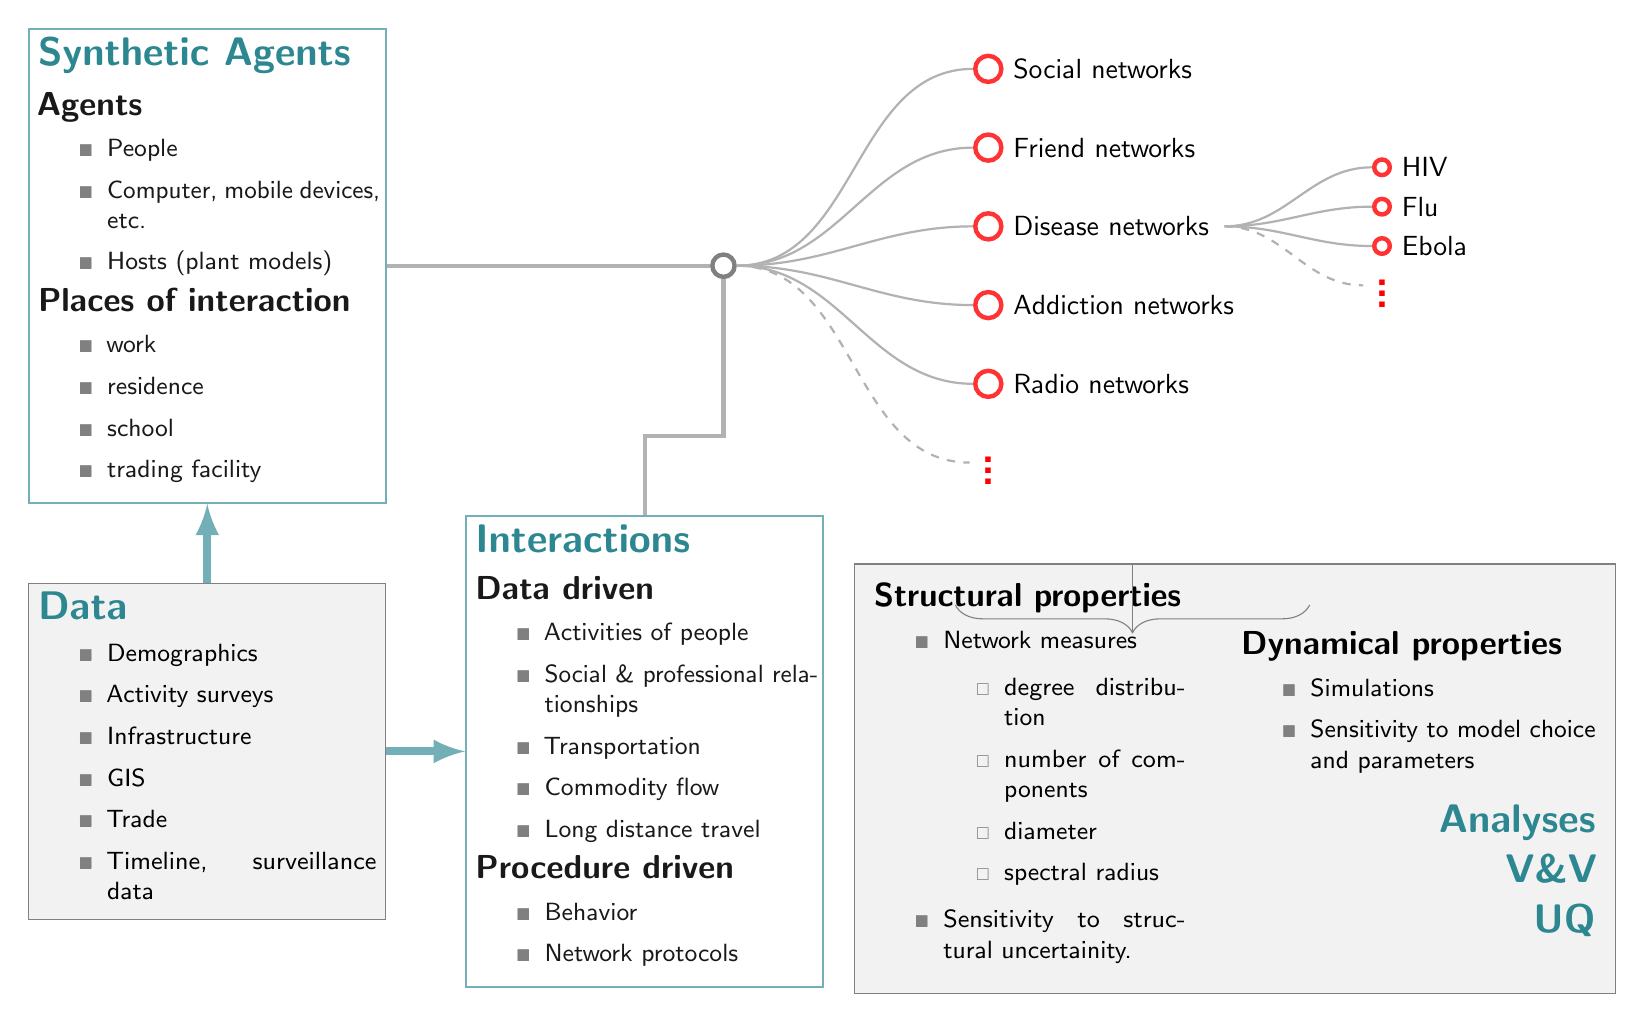
\begin{tikzpicture}
[scale=1,auto, transform shape,
%% show background rectangle,
%% background rectangle/.style={fill=white},
every node/.style={align=left},
titleblock/.style={font=\large,font=\bf,rectangle,minimum width=1cm,text=white,fill=black!50},
descblock/.style={font=\small,black!90,draw=DarkBlue,thick,rectangle,minimum width=2cm},
grayblock/.style={font=\small,black,draw=gray,fill=gray!10,rectangle,minimum width=2cm},
netblock/.style={font=\small,black!80,draw=red!80,ultra thick,circle,minimum width=.1cm},
dblock/.style={font=\small,black!80,draw=red!80,ultra thick,circle,inner
   sep=.07cm},
anc/.style={shape=circle,inner sep=3pt,fill=black},
thickedge/.style={>=latex, shorten >=.0pt, shorten <=.0pt, 
line width=1mm},
cedge/.style={gray!60,>=latex', shorten >=.0pt, shorten <=.0pt, 
thick},
specedge/.style={draw=red!40,>=latex', shorten >=.0pt, shorten <=.0pt},
iedge/.style={draw=black,>=latex', shorten >=.0pt, shorten <=.0pt, ultra
thick, dashed}]
%%%%%%%%%%%%%%%%%%%%%%%%%%%%%%%%%%%%%%%%%%%%%%%%%%%%%%%%%%%%%%%%%%%%%%%%%%%
%% Digital library
%%%%%%%%%%%%%%%%%%%%%%%%%%%%%%%%%%%%%%%%%%%%%%%%%%%%%%%%%%%%%%%%%%%%%%%%%%%
\node (data) [grayblock,minimum width=4.5cm]{\parbox{4.3cm}{
%%\colorbox{DarkBlue}{\textcolor{white}{Digital library}}
{\textcolor{DarkBlue!150}{\Large\bfseries Data}}
\begin{itemize}
\item Demographics
\item Activity surveys
\item Infrastructure
\item GIS
\item Trade
\item Timeline, surveillance data
\end{itemize}}};
%%
%% \node (construct) [descblock,minimum width=4.5cm,draw=DarkBlue,above=of
%% data]{\parbox{4.3cm}{
%% %%\colorbox{DarkBlue}{\textcolor{white}{Digital library}}
%% {\textcolor{DarkBlue!150}{Construction methods}}
%% \vspace{.2cm}
%% \begin{itemize}
%% \item
%% \item
%% \item
%% \end{itemize}}};
%%
\node (synthpop) [descblock,minimum width=4.5cm,above=of data,shift={(0,0)}]{\parbox{4.3cm}{
%%\colorbox{DarkBlue}{\textcolor{white}{Digital library}}
   {\textcolor{DarkBlue!150}{{\Large\bfseries Synthetic Agents}}}
\vspace{.2cm}\\
\textbf{\large Agents}
\begin{itemize}
\item People
\item Computer, mobile devices, etc.
\item Hosts (plant models)
\end{itemize}
\textbf{\large Places of interaction}
\begin{itemize}
\item work 
\item residence 
\item school 
\item trading facility
\end{itemize}}};
%%
\node (interactions) [descblock,minimum width=4.5cm,right
=of data,shift={(0,0)}]{\parbox{4.3cm}{
%%\colorbox{DarkBlue}{\textcolor{white}{Digital library}}
{\textcolor{DarkBlue!150}{\Large\bfseries Interactions}}\vspace{.2cm}\\
\textbf{\large Data driven}
\begin{itemize}
\item Activities of people
\item Social \& professional relationships
\item Transportation
\item Commodity flow
\item Long distance travel
\end{itemize}
%%
\textbf{\large Procedure driven}
\begin{itemize}
\item Behavior
\item Network protocols
\end{itemize}}};
%%
\node (anc1) [circle,fill=white,draw=gray,ultra thick,shift={(1,0)},inner sep=.1cm] at (interactions|-synthpop) {};
%%
\node (radionet) [netblock,right=of anc1,shift={(2,-1.5)},label=right:Radio
networks]{};
\node (addictionnet) [netblock,above of=radionet,label=right:Addiction
networks]{};
\node (contactnet) [netblock,above of=addictionnet,label=right:Disease
networks]{};
\node (friendsnet) [netblock,above of=contactnet,label=right:Friend
networks]{};
\node (socialnet) [netblock,above of=friendsnet,label=right:Social networks]{};
networks]{};
\node (miscnet) [below of=radionet,red,font=\Huge] {$\vdots$};
%%
\node (hiv) [dblock,right of=contactnet,shift={(4,.75)},label=right:HIV] {};
\node (flu) [dblock,below of=hiv,shift={(0,.5)},label=right:Flu] {};
\node (ebola) [dblock,below of=flu,shift={(0,.5)},label=right:Ebola] {};
\node (misc) [below of=ebola,shift={(0,.5)},,red,font=\Huge] {$\vdots$};
%%
%%%%%%%%%%%
%% Arrows
%%%%%%%%%%%
\draw[thickedge,DarkBlue,->] (data) -- (synthpop);
\draw[thickedge,DarkBlue,->] (data) -- (interactions.west|-data);
\draw[cedge,ultra thick] (synthpop) edge[out=0,in=180] (anc1);
\draw[cedge,ultra thick] (interactions.north) -- ++(0,1) -| (anc1);
\draw[cedge] (anc1) edge[out=0,in=180] (contactnet);
\draw[cedge] (anc1) edge[out=0,in=180] (socialnet);
\draw[cedge] (anc1) edge[out=0,in=180] (radionet);
\draw[cedge] (anc1) edge[out=0,in=180] (friendsnet);
\draw[cedge] (anc1) edge[out=0,in=180] (addictionnet);
\draw[cedge,dashed] (anc1) edge[out=0,in=180] (miscnet);
%%
\draw[cedge] (contactnet)++(3,0) edge[out=0,in=180] (hiv);
\draw[cedge] (contactnet)++(3,0) edge[out=0,in=180] (flu);
\draw[cedge] (contactnet)++(3,0) edge[out=0,in=180] (ebola);
\draw[cedge,dashed] (contactnet)++(3,0) edge[out=0,in=180] (misc);
%% %%
%% %% Net specific
%% %%
%% \begin{pgfonlayer}{background}
%% \draw[specedge] (contactnet) -- ++(-.25,.25) -- ++(0,1.2) -- ++(.6,0);
%% \draw[specedge] (socialnet) -- ++(-.45,.45) -- ++(0,2.4) -- ++(.8,0);
%% \draw[specedge] (radionet) -- ++(-.65,.65) -- ++(0,3.6) -- ++(1,0);
%% \end{pgfonlayer}
%%
%% big triangle
%%
%% \begin{scope}[shift={(16,-.5)},local bounding box=bigTriangle]
%% \fill[black!30] (0,0) -- (0,4) -- (.5,2) -- cycle;
%% \end{scope}
%%
%% \node (app) [descblock,right=of bigTriangle,draw=DarkBlue] {Applications};
%%%%%%%%%%%
% V&V
%%%%%%%%%%%
\node (netvv) [descblock,black,draw=none,minimum width=4cm,below= of
miscnet,shift={(.5,0)}] {\parbox{3.9cm}{
   {\large\bfseries Structural properties}
   \begin{itemize}
      \item Network measures
      \begin{itemize}
         \item degree distribution
         \item number of components
         \item diameter
         \item spectral radius
      \end{itemize}
      \item Sensitivity to structural uncertainity.
   \end{itemize}}};
%%
\node (dynvv) [descblock,black,draw=none,minimum width=4.5cm,right= of
netvv,shift={(-.5,.9)}] {\parbox[][][t]{4.5cm}{
   {\large\bfseries Dynamical properties}
   \begin{itemize}
      \item Simulations
      \item Sensitivity to model choice and parameters
   \end{itemize}
}};
\begin{pgfonlayer}{background}
\node (vv)
[grayblock,fill=gray!10,fit=(dynvv)(netvv)]{};
\end{pgfonlayer}
\node (vvtitle) [descblock,draw=none,DarkBlue!150,below=of dynvv,shift={(0,1)}]
{\parbox{4.5cm}{\raggedleft\bfseries\Large 
Analyses \\ V\&V\\ UQ}};
%%
%% \draw[specedge,gray] (anc1) -- ++(0,-2) -| (dynvv);
\draw [shift={(9.5,3.5)},gray,decorate,decoration={brace,amplitude=10pt,mirror,raise=4pt},yshift=0pt]
(0,-1.5) -- (4.5,-1.5) node (brace) [midway,below,yshift=-.5cm,black] {};
\draw[specedge,gray] (brace)+(0,.15) -- (vv.north-|brace);
\end{tikzpicture}
\end{document}
